% inspired from http://tex.stackexchange.com/questions/63612/tikz-tree-drawing-with-comments-to-each-level
\documentclass{article}

\usepackage{tikz}
\usetikzlibrary{trees}

\begin{document}

% Exemple arbre

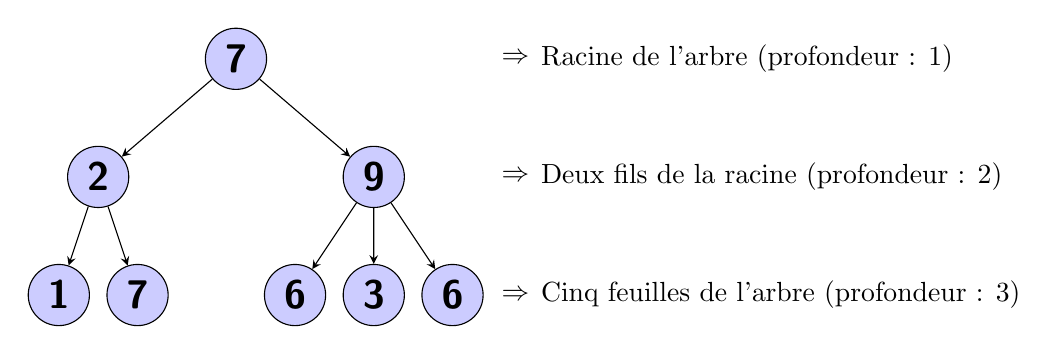
\begin{tikzpicture}[level distance = 1.5cm,
         level 1/.style = {->, >=stealth, sibling distance = 3.5cm},
         level 2/.style = {->, >=stealth, sibling distance = 1cm}]
\tikzstyle{every node} = [circle, fill = blue!20, draw, font = \sffamily\Large\bfseries]
\node (Root) {7}
   child {
      node {2}
      child { node {1} }
      child { node {7} }
   }
   child {
      node {9}
      child { node {6} }
      child { node {3} }
      child { node {6} }
   };

   \begin{scope}[every node/.style = {right}]
      \path (Root    -| Root-2-3) ++(5mm,0) node {$\Rightarrow$} ++(5mm,0) node {Racine de l'arbre (profondeur : 1)};
      \path (Root-1  -| Root-2-3) ++(5mm,0) node {$\Rightarrow$} ++(5mm,0) node {Deux fils de la racine (profondeur : 2)};
      \path (Root-1-1-| Root-2-3) ++(5mm,0) node {$\Rightarrow$} ++(5mm,0) node {Cinq feuilles de l'arbre (profondeur : 3)};
   \end{scope}

\end{tikzpicture}

\end{document}
